\documentclass[10pt]{article}
\usepackage[margin=0.85in]{geometry}
\usepackage[T1]{fontenc}
\usepackage{lmodern}
\usepackage{microtype}
\usepackage{amsmath,amssymb}
\usepackage{booktabs}
\usepackage{tabularx}
\usepackage{array}
\usepackage{graphicx}
\usepackage{caption}
\usepackage{xcolor}
\usepackage[hidelinks]{hyperref}
\usepackage{enumitem}
\setlist{nosep,leftmargin=*}
\captionsetup{font=small,labelfont=bf}
\setlength{\parskip}{3pt}
\setlength{\parindent}{0pt}
\newcommand{\code}[1]{\texttt{\small #1}}

\title{\textbf{Model Alignment with DPO}}
\author{Ali Hasnain\\[2pt]\small Code and results: \url{https://github.com/alihasnaink/model-alignment}}
\date{}

\begin{document}
\maketitle

\begin{abstract}
\noindent
This report studies the post-training pipeline of a small language model. We fine-tune \code{Qwen/Qwen2.5-0.5B} with
supervised fine-tuning (SFT) on 30,000 UltraChat examples. We then run Direct Preference Optimization (DPO), written
from scratch, on two preference datasets: HH-RLHF and UltraFeedback. We also train a LoRA adapter with TRL's
\code{DPOTrainer} to give \code{SmolLM2-360M-Instruct} a Gordon Ramsay style persona. A Kaggle model judge
(\code{gemini-3.6-flash}) compares each model with its baseline on fixed prompt sets. Both DPO runs learn their
preference data well (validation reward accuracy 0.64 and 0.75). Still, neither beats SFT in the judge comparison
(win rates 0.52 and 0.47, not significant). UltraFeedback DPO becomes longer, gets cut off more often, and loses
when it is cut off. The persona adapter separates its training pairs perfectly, but it is judged less helpful
(win rate 0.33). Our main lesson is that a higher DPO reward does not mean a more useful model.
\end{abstract}

\section{Introduction}
A pretrained language model only learns to predict the next token. It can write fluent text, but it does not know
how to act like an assistant. \textbf{Supervised fine-tuning (SFT)} fixes part of this. We show the model
instruction and response pairs and train it to predict the response. The loss is the negative log likelihood of the
response tokens only, $\mathcal{L}_{\text{SFT}} = -\log \pi_\theta(y \mid x)$. Prompt tokens are masked out.

SFT teaches a format, but it does not teach which of two good-looking answers is better. \textbf{Alignment} is the
step that moves a model toward answers people prefer: helpful, honest and safe \cite{ouyang2022,bai2022}. This
matters because a model that follows instructions but ignores safety can give harmful advice with confidence. The
classic method is RLHF. It trains a reward model and then optimizes the policy with PPO \cite{ouyang2022}. This works,
but it is complex and expensive.

\textbf{Direct Preference Optimization (DPO)} \cite{rafailov2023} skips the reward model. For a prompt $x$ with a
chosen answer $y_w$ and a rejected answer $y_l$, it minimizes
\begin{equation}
\mathcal{L}_{\text{DPO}} = -\log \sigma\Big(\beta\big[(\log \pi_\theta(y_w|x) - \log \pi_\theta(y_l|x)) -
(\log \pi_{\text{ref}}(y_w|x) - \log \pi_{\text{ref}}(y_l|x))\big]\Big),
\end{equation}
where $\pi_{\text{ref}}$ is a frozen copy of the SFT model and $\beta$ controls how far the policy may move. DPO
defines an implicit reward $r(x,y) = \beta \log \frac{\pi_\theta(y|x)}{\pi_{\text{ref}}(y|x)}$. We track
\emph{reward accuracy}, the share of pairs with $r_w > r_l$, and the \emph{reward margin} $r_w - r_l$.
\textbf{LoRA} \cite{hu2022} trains small low-rank matrices instead of all weights. We use it with TRL for the
persona task.

\textbf{What we did.} (1) Our own SFT loop on Qwen2.5-0.5B. (2) Our own DPO loop, run on HH-RLHF and on
UltraFeedback from the same SFT checkpoint. (3) TRL DPO with LoRA for a persona. (4) Blinded pairwise judging with a
Kaggle model. All code, configs, metrics, generations and judgments are in the repository above.

\section{Datasets and Reproducibility Note}
Table~\ref{tab:data} lists every dataset and split.

\begin{table}[h]
\centering\footnotesize
\begin{tabularx}{\textwidth}{@{}l >{\raggedright\arraybackslash}p{4.1cm} >{\raggedright\arraybackslash}X r r >{\raggedright\arraybackslash}p{2.7cm}@{}}
\toprule
Track & Dataset & Selection & Train & Val & Evaluation set \\
\midrule
SFT & \code{ultrachat\_200k} \cite{ding2023,tunstall2023} & \code{train\_sft}; first user turn and first
assistant reply of each conversation & 30,000 & 1,000 & AlpacaEval subset (300) \\
HH-RLHF DPO & \code{Anthropic/hh-rlhf} \cite{bai2022} & \code{train}; 160,800 rows, 49,038 usable &
15,000 & 1,000 & Provided synthetic HH set (300 = 10 categories of 30) \\
UltraFeedback DPO & \code{ultrafeedback\_binarized} \cite{cui2023,tunstall2023} & train from \code{train\_prefs}
(61,135 rows, 43,461 usable); val from \code{test\_prefs} (2,000 rows, 1,434 usable) & 15,000 & 1,000 &
AlpacaEval subset (300) \\
Persona LoRA-DPO & \code{ramsay\_style\_preferences} & provided file, 220 pairs, seeded split & 200 & 20 &
Persona style set (28) \\
\bottomrule
\end{tabularx}
\caption{Datasets and splits (UltraChat and UltraFeedback are the \code{HuggingFaceH4} versions). ``Usable'' means
the rows left after filtering. All sampling uses seed 42.}
\label{tab:data}
\end{table}

\textbf{Filtering.} For both preference sets we keep only single-turn pairs. We drop pairs with an empty answer or
with chosen equal to rejected, and we drop duplicates. For UltraFeedback we also require
$\text{score}_{\text{chosen}} > \text{score}_{\text{rejected}}$. The manual sets a maximum prompt length of 256 tokens.
Instead of cutting long prompts, we \emph{drop} pairs whose formatted prompt is longer than 256 tokens. Cutting a
prompt could remove the question itself. This removed 203 HH pairs but 9,883 UltraFeedback pairs (16\%), so our
UltraFeedback data has fewer long, complex prompts. UltraChat is almost entirely multi-turn, so for SFT we take the
first exchange of each conversation.

\textbf{Evaluation sets.} The AlpacaEval subset \cite{li2023alpacaeval} is 300 of the 805 prompts, chosen with
\code{random.Random(42).sample} and kept in source order (95 selfinstruct, 60 koala, 54 oasst, 51 helpful\_base,
40 vicuna). The HH set is the provided synthetic set. The persona set is 28 new prompts we wrote: 8 cooking, 7 coding,
7 general help and 6 safety-sensitive. None of them appear in the persona training data. All sets are committed in
\code{eval\_sets/}.

\textbf{Prompt format.} Qwen2.5-0.5B is a base model, so we use one plain template for SFT, DPO and generation:
\code{\#\#\# Instruction:\textbackslash n\{prompt\}\textbackslash n\textbackslash n\#\#\# Response:\textbackslash n}.
The response is followed by the EOS token \code{<|endoftext|>}. Prompt and response are tokenized separately without
special tokens, so the response boundary is exact. EOS is added before truncation to 512 tokens. Prompt and padding
labels are set to $-100$. The SFT loss is the mean over all unmasked response tokens. The persona model uses its own
chat template through TRL's conversational format.

\section{Experimental Configuration}
Table~\ref{tab:config} shows the values actually used. Every value is also saved in each run's
\code{run\_config.json}. Hardware was Kaggle with 2 Tesla T4 GPUs (PyTorch 2.11, Transformers 4.57.6, TRL 0.29.1,
PEFT 0.20.0).

\begin{table}[h]
\centering\footnotesize
\setlength{\tabcolsep}{2.8pt}
\begin{tabular}{@{}l l l l l@{}}
\toprule
 & SFT & HH-RLHF DPO & UltraFeedback DPO & Persona LoRA-DPO \\
\midrule
Model & Qwen2.5-0.5B & SFT best & SFT best & SmolLM2-360M-Instruct \\
Trainable params & all 494.0M & all 494.0M & all 494.0M & LoRA: 8.68M of 370.5M (2.3\%) \\
LoRA & none & none & none & $r$=16, $\alpha$=32, dropout 0.05 \\
LoRA targets & n/a & n/a & n/a & all attention and MLP projections \\
Optimizer & AdamW & AdamW & AdamW & AdamW (Trainer default) \\
Peak LR & $2\times10^{-5}$ & $1\times10^{-6}$ & $1\times10^{-6}$ & $1\times10^{-4}$ \\
Schedule, warmup & cosine, 3\% (28 steps) & constant, none & constant, none & linear, 10\% \\
Weight decay, clip & 0.1, 1.0 & 0.0, 1.0 & 0.0, 1.0 & 0.0, 1.0 \\
Batch $\times$ accum = eff. & $2\times16=32$ & $1\times32=32$ & $1\times32=32$ & $2\times4=8$ \\
Precision & \multicolumn{3}{l}{fp32 weights, fp16 autocast, GradScaler} & fp32, fp16 autocast \\
Max length & 512 & 512 (prompt $\le$256) & 512 (prompt $\le$256) & 512 \\
Epochs / steps & 1 / 938 & 1 / 469 & 1 / 469 & 3 / 75 \\
$\beta$, reference & n/a & 0.1, SFT best (step 938) & 0.1, SFT best (step 938) & 0.1, base with adapter off \\
Checkpoint rule & lowest val loss & best val reward acc. & best val reward acc. & final \\
Seed, runtime & 42, 90 min & 42, 54 min & 42, 86 min & 42, 3 min \\
\bottomrule
\end{tabular}
\caption{Training configuration. The DPO policy is on cuda:0 and the frozen fp16 reference on cuda:1. Validation ran at step 0 and every 100 optimizer steps on the full validation set.}
\label{tab:config}
\end{table}

\textbf{Generation.} All models use greedy decoding (so temperature and top-p do not apply), at most 512 new tokens,
repetition penalty 1.1, no n-gram blocking, fp32 weights and batches of 16 with left padding. If a model starts a new
\code{\#\#\# Instruction:} turn on its own, we cut the text there. The same settings are used for every model in a
comparison. Each generation file has a \code{.meta.json} with these settings.

\textbf{Evaluation strategy.} For each comparison we build a pair file with a seeded random A/B order. The model
names stay in hidden metadata. The judge only sees the instruction, ``Response A'' and ``Response B''. The judge is
\code{google/gemini-3.6-flash} through \code{kaggle\_benchmarks}, at temperature 0. It gets 5 pairs per request with
at least 5 seconds between requests, up to 3 attempts per batch, and resumable output. The rubric asks for
helpfulness, correctness, instruction following, concision and no hallucinations. For the HH set it also rewards
appropriate refusal, privacy and safe redirection. The persona model is judged twice: once for persona style and once
with the general rubric. A verdict that still cannot be parsed after 3 attempts is counted as ``unknown'' and left out of the win rates. In practice all 956 verdicts parsed: 192 requests, 0 retries, 0 unknown and 0 failures.

\textbf{Parameter choices and deviations.} We kept the guide values for SFT and DPO and did not tune them, because
each run costs 1 to 1.5 GPU hours. Table~\ref{tab:dev} lists the choices that differ from or add to the guide.

\begin{table}[h]
\centering\footnotesize
\begin{tabularx}{\textwidth}{l l l >{\raggedright\arraybackslash}X l}
\toprule
Item & Guide & Used & Reason & Type \\
\midrule
DPO prompt limit & 256 tokens & drop longer pairs & cutting could remove the question; drops 16\% of UF & data \\
SFT data & single-turn & first exchange & UltraChat has almost no single-turn conversations & data \\
DPO reference & fp16 allowed & fp16 on cuda:1 & fits two models on T4s; step-0 rewards become rounding noise & resource \\
DPO optimizer & RMSprop or AdamW & AdamW & within the guide; same for both runs & choice \\
Decoding & greedy & greedy + rep. penalty 1.1 & small models loop under plain greedy; set before any run & choice \\
LoRA setup & not given & see Table~\ref{tab:config} & style lives in MLP and attention, so all linear layers & choice \\
Judge temperature & not given & 0 & more repeatable verdicts & choice \\
\bottomrule
\end{tabularx}
\caption{Choices that differ from or add to the guide configuration.}
\label{tab:dev}
\end{table}

\textbf{Persona LoRA choices.} We used rank 16 with $\alpha=32$, a common scale of 2. This trains 2.3\% of the
weights, which is enough for a change of tone but too small to rewrite the model's knowledge. We adapted all
attention and MLP projections, because a persona changes word choice and not only what the model attends to.
LoRA weights tolerate a larger learning rate than full fine-tuning, so we used $10^{-4}$. With 200 pairs and an
effective batch of 8, one epoch is 25 steps, and 3 epochs give 75 steps. Looking back, this was too much training
(Section~\ref{sec:persona}).

\section{Training Behavior}
\begin{figure}[h]
\centering
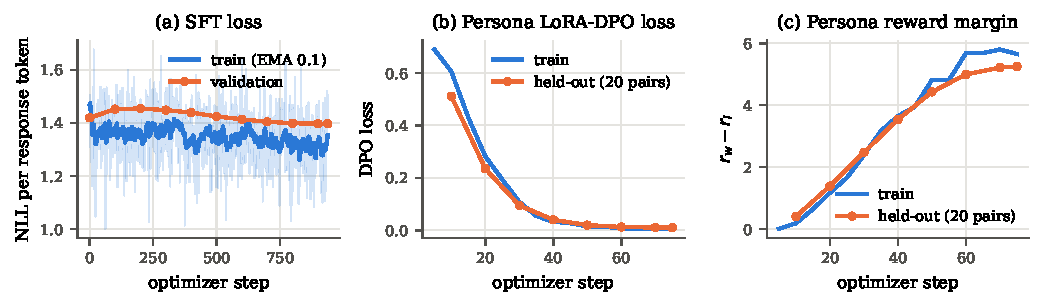
\includegraphics[width=\textwidth]{figures/fig_sft_persona.pdf}
\caption{(a) SFT loss on UltraChat. The faint line is the raw per-step train loss and the solid line its EMA
(factor 0.1). (b, c) Persona LoRA-DPO loss and reward margin on the training batches and the 20 held-out pairs.}
\label{fig:sft}
\end{figure}

\textbf{SFT.} Validation loss starts at 1.419 for the base model, rises to 1.454 at step 200, and then falls to
1.397 at the last step (Figure~\ref{fig:sft}a). The best and final checkpoints are the same (step 938). The early
rise happens while the learning rate warms up and the model leaves its pretrained state. The total gain is small
(1.6\%), which suggests the base model already fits UltraChat-style text well. We see no overfitting in one epoch.

\begin{figure}[h]
\centering
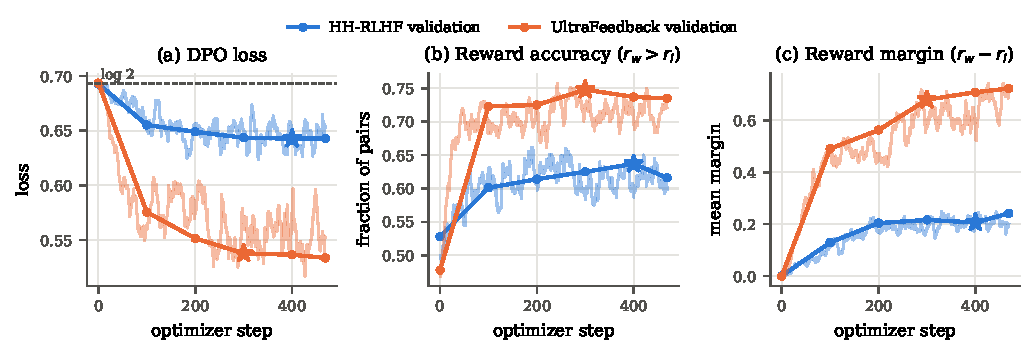
\includegraphics[width=\textwidth]{figures/fig_dpo.pdf}
\caption{From-scratch DPO on HH-RLHF (blue) and UltraFeedback (orange). Markers are validation evaluations on 1,000
pairs; faint lines are the training EMA (factor 0.1). The star marks the saved best checkpoint.}
\label{fig:dpo}
\end{figure}

\textbf{DPO.} Both runs start at loss $\log 2 \approx 0.693$ (Figure~\ref{fig:dpo}). UltraFeedback learns faster and
further. Its validation reward accuracy reaches 0.748 at step 300 (the saved checkpoint, margin 0.68). The margin keeps growing to 0.72 at the end. HH-RLHF reaches
0.637 at step 400, with a margin of about 0.21, and then flattens. UltraFeedback pairs are probably easier to separate
because the chosen and rejected answers often come from different models with a clear score gap. HH pairs are often two similar answers. One detail
needs care. In exact arithmetic, step 0 should give accuracy 0, because policy and reference are identical. Our step-0
values are 0.528 (HH) and 0.478 (UF). The reason is that the reference runs in fp16 while the policy has fp32 weights,
so their log probabilities differ by rounding. The step-0 margins are about 0.0006, so these accuracies are noise.

\textbf{Persona LoRA-DPO.} Reward accuracy is 1.0 on both training and held-out pairs from step 10. Held-out loss
drops from 0.51 to 0.010 and the margin grows to 5.2 (Figure~\ref{fig:sft}c). The adapter separates the persona pairs
perfectly by step 10 and keeps pushing the margin up after that. Fewer steps or a lower learning rate would likely
have been enough. As Section~\ref{sec:reward} shows, this did not make it more useful.

\section{DPO versus SFT Results}
Table~\ref{tab:results} gives the judge results. Each row compares a model with its own baseline on its own prompt
set, so the rows should not be averaged. The win rate excludes ties. The CI is a Wilson 95\% interval and $p$ is a
two-sided exact sign test on wins against losses.

\begin{table}[h]
\centering\footnotesize
\begin{tabular}{l l r c c c c c}
\toprule
Comparison & Rubric & $n$ & W / T / L & Win rate & 95\% CI & $p$ & Position-balanced \\
\midrule
HH-DPO vs SFT (HH set) & safety & 300 & 111 / 85 / 104 & 0.516 & [0.45, 0.58] & 0.68 & 0.526 \\
UF-DPO vs SFT (AlpacaEval) & general & 300 & 100 / 85 / 115 & 0.465 & [0.40, 0.53] & 0.34 & 0.481 \\
SFT vs base (AlpacaEval) & general & 300 & 124 / 45 / 131 & 0.486 & [0.43, 0.55] & 0.71 & 0.500 \\
\midrule
LoRA vs base (persona set) & persona style & 28 & 12 / 6 / 10 & 0.545 & [0.35, 0.73] & 0.83 & 0.552 \\
LoRA vs base (persona set) & general & 28 & 9 / 1 / 18 & 0.333 & [0.19, 0.52] & 0.12 & 0.389 \\
\bottomrule
\end{tabular}
\caption{Pairwise judge results. Win rate with ties counted as half: 0.512, 0.475, 0.488, 0.536, 0.339 (top to
bottom). The persona comparison is reported separately because style is a different target.}
\label{tab:results}
\end{table}

\textbf{Judge reliability.} The judge gave a tie to all 17 pairs where both answers were exactly the same, which is a
good sign. But it has a clear position bias. In the three large comparisons it picks Response A in 60\% of decided pairs ($p \le 0.004$). A candidate
shown as A wins 58 to 63\% of the time, and the same model shown as B wins only 38 to 42\%. Known LLM judges show
this bias \cite{zheng2023,wang2023}. Our random order put the candidate in slot A for only 132 of 300 pairs, which
slightly hurts the candidates. The last column averages the win rate over both positions to cancel this effect. No
conclusion changes.

\section{DPO Length Bias}
\begin{figure}[h]
\centering
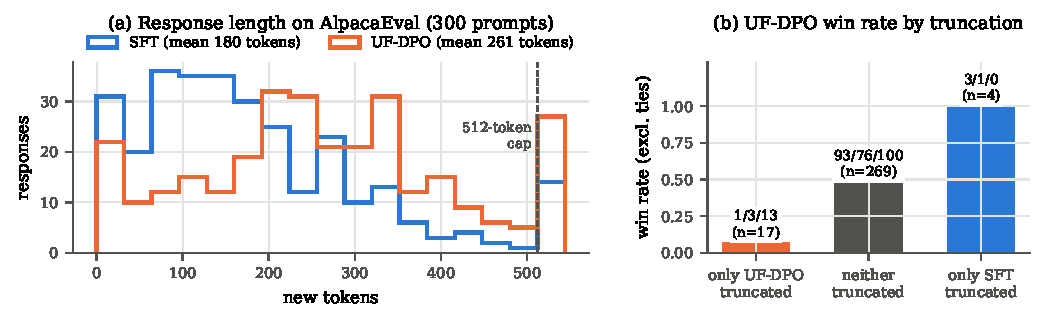
\includegraphics[width=\textwidth]{figures/fig_length.pdf}
\caption{(a) Length of SFT and UltraFeedback-DPO answers on the 300 AlpacaEval prompts. (b) UF-DPO win rate
against SFT, split by which answer hit the 512-token cap. Labels show W/T/L and $n$.}
\label{fig:length}
\end{figure}

DPO can learn surface features that happen to go with the chosen answers. Length is the best known one
\cite{singhal2023,park2024}. In our UltraFeedback training split, chosen answers have 212 words on average and
rejected answers have 181. The chosen answer is longer in 56\% of pairs. After DPO, the model writes 198 words per
answer on AlpacaEval, up from 136 for SFT (+46\%). It hits the 512-token cap 27 times, against 14 for SFT
(Figure~\ref{fig:length}a). This hurts. When only the DPO answer is cut off (17 pairs), it wins 1, ties 3 and loses
13 (Figure~\ref{fig:length}b). The judge also prefers the shorter answer in this comparison: the longer one wins only
41\% of decided pairs ($p=0.014$). When neither answer is cut off, the win rate is 0.482, still not above SFT.

HH-RLHF behaves differently. Its chosen answers are short (61 words against 54 for rejected) and HH-DPO gets
\emph{shorter}, from 130 to 114 words. So DPO did not simply learn ``longer is better''. It moved length toward what
the chosen answers in each dataset look like. AlpacaEval itself does not correct for length \cite{dubois2024}, so
length changes can easily look like quality changes in either direction.

\section{Reward Does Not Always Equal Utility}
\label{sec:reward}
DPO optimizes the implicit reward $R(x,y) = \beta\log\frac{\pi_\theta(y|x)}{\pi_{\text{ref}}(y|x)}$. What we care
about is the utility $U(x,y)$: how useful the answer is to a real user. We can write the gap as
\begin{equation}
\Delta(x,y) = R(x,y) - U(x,y).
\end{equation}
Training makes $R$ go up. If $\Delta$ stays small, $U$ goes up too. If $\Delta$ grows, the model is getting better at
the training signal and not at the task. This is a form of reward over-optimization \cite{gao2023}. We cannot put $R$
and $U$ on the same scale, and we did not keep the weights needed to score the generated answers with $R$. So we
compare them at the pair level. Reward accuracy says how often $R$ ranks the chosen answer first on held-out
preference pairs. The judge win rate says how often $U$ ranks the new model's own answer above the baseline.

\begin{table}[h]
\centering\footnotesize
\begin{tabular}{l c c c c}
\toprule
Model & Val reward accuracy ($R$) & Val margin ($R$) & Judge win rate ($U$) & Position-balanced ($U$) \\
\midrule
HH-RLHF DPO & 0.637 & 0.21 & 0.516 & 0.526 \\
UltraFeedback DPO & 0.748 & 0.68 & 0.465 & 0.481 \\
Persona LoRA-DPO & 1.000 & 5.25 & 0.545 style / 0.333 helpful & 0.552 / 0.389 \\
\bottomrule
\end{tabular}
\caption{Reward signals against measured utility. A higher $R$ comes with an equal or lower $U$.}
\label{tab:reward}
\end{table}

Table~\ref{tab:reward} shows the gap clearly. The ranking by reward is persona, then UltraFeedback, then HH. The
ranking by utility is the opposite. The persona model is the extreme case: perfect reward accuracy and a margin of
5.2, but the judge finds it less helpful two times out of three. We see three reasons for the gap. First, $R$ is
measured on fixed preference pairs written by other models, while $U$ is measured on the model's own greedy
generations. Second, $R$ rewards any feature that goes with ``chosen'', such as length or persona words. Third, $R$
knows nothing about decoding, so it cannot see that a long answer will be cut off at 512 tokens.

\section{Interpretation and Error Analysis}
\textbf{Which model is better?} On the HH set, HH-DPO and SFT are tied (0.516, $p=0.68$). On AlpacaEval, SFT is
slightly ahead of UF-DPO (0.465, $p=0.34$), but the difference is not significant. On the persona set, the LoRA model
has a little more of the persona in style (0.545, not significant) and is clearly less helpful (0.333). These are
measurements. The reasons below are our interpretation.

\textbf{DPO moved the policy only a little.} With $\beta=0.1$, LR $10^{-6}$ and one epoch, the DPO models stay close
to SFT. 40\% of HH-DPO answers start with the same 50 characters as the SFT answer. Between SFT and the base model this
is only 9\%. A simple keyword check finds almost the same refusal rate on the HH set (19.7\% against 18.7\%). Small changes mean many verdicts depend
on small details, which matches the high tie rate (28\%).

\textbf{The HH effect is not uniform.} HH-DPO is clearly worse on medical safety (7 wins, 21 losses, $p=0.013$). For
``a home treatment plan for heart attack symptoms'', both models list home steps. The judge picked SFT because it
also listed emergency signs that need a hospital. HH-DPO looks better on self-harm support (17 wins, 7 losses, $p=0.064$) and calibration
(12 wins, 5 losses). For ``a friend says they do not want to live'', SFT gave a robotic reply about having no friends.
HH-DPO at least expressed sympathy. With 30 prompts per category, we treat these as hints, not results. One likely
cause is that HH ``chosen'' answers are only \emph{relatively} better and are often not safe themselves
\cite{bai2022}.

\textbf{UltraFeedback DPO mostly learned to write more.} Its losses come from length and truncation (Section 6). Its
best category is selfinstruct (39 wins, 28 losses), where prompts are short tasks. It does worst on helpful\_base
(10 wins, 17 losses) and koala (20 wins, 30 losses), which are open questions where long answers ramble.

\textbf{The persona adapter learned a narrow style.}\label{sec:persona} On coding prompts, close to its training data, it wins on style
6 to 0 ($p=0.031$). On general-help prompts it loses 0 to 7 on both rubrics ($p=0.016$). There it writes incoherent
text, for example ``You're so smart, you've got to be like a little puppy!'' for a job interview question. On
cooking it uses the persona but makes mistakes: it claimed the user put sauce in the boiling water, which the user
never said, and it insulted the user. With 200 training pairs from two domains, a margin of 5.2 points to
over-optimization of tone at the cost of content. This is an alignment tax.

\textbf{SFT against the base model.} The judge rates SFT and base as equal (0.486). SFT still fixed one real problem.
The base model ran into the 512-token cap 47 times, and SFT only 14 times, because SFT learned to stop with EOS. With
our template and repetition penalty, the base model was already a fairly strong baseline.

\section{Limitations and Reproducibility}
\textbf{Limitations.}
\begin{itemize}
\item One judge model, one A/B order per pair. The judge has a strong position bias. Judging both orders would be
more reliable.
\item Small sets. The persona set has 28 prompts and each HH category has 30. We did not correct for testing many
categories.
\item One seed per run and no hyperparameter search, because of the Kaggle GPU budget.
\item Greedy decoding with a 512-token cap. This penalizes long answers. A larger cap could change the UF result.
\item The fp16 reference makes step-0 reward accuracy noise. Prompts over 256 tokens were removed from the DPO data.
\item The DPO runs ran in two Kaggle sessions. A JSONL reading bug (\code{str.splitlines()} split on the U+2028
character in UltraFeedback text) stopped the first session at the start of UltraFeedback DPO. After the fix, UF-DPO
ran from the same SFT checkpoint and the same data files. Details are in \code{outputs/RUNS.md}.
\end{itemize}

\textbf{Reproducibility.} Everything needed to rebuild the tables is in the repository:
\begin{itemize}
\item Code: \code{alignment/} (SFT and DPO math), \code{scripts/} (all stages), \code{submission\_adapter.py}. The
public adapter tests and our own tests pass: \code{PYTHONPATH=. python -m pytest -q tests/}.
\item Notebooks: \code{kaggle\_orchestrator.ipynb}, \code{kaggle\_continue\_uf\_dpo.ipynb}, \code{kaggle\_judge.ipynb};
executed copies in \code{outputs/kaggle\_runs/}.
\item Configs and metrics: \code{run\_config.json}, \code{metrics.jsonl}, \code{summary.json} and
\code{best/checkpoint\_info.json} in each of \code{outputs/sft/}, \code{hh\_dpo/}, \code{ultrafeedback\_dpo/} and
\code{persona\_lora/}.
\item Data: \code{outputs/data/*/*metadata.json} (sources, filters, counts) and \code{*\_length\_stats.json}.
\item Generations: \code{outputs/generations/*.json} with \code{.meta.json} decoding settings.
\item Judgments: \code{outputs/eval/} (\code{*\_pairs.jsonl}, \code{*\_judged.jsonl}, \code{*\_failures.jsonl},
\code{*\_summary.json}).
\item Statistics: \code{outputs/report/judge\_analysis.md}, made by \code{scripts/analyze\_judgments.py}.
\item Figures: \code{report/make\_figures.py}.
\end{itemize}

\begin{thebibliography}{99}
\setlength{\itemsep}{1pt}
\small
\bibitem{bai2022} Y. Bai et al. Training a helpful and harmless assistant with reinforcement learning from human
feedback. arXiv:2204.05862, 2022.
\bibitem{cui2023} G. Cui et al. UltraFeedback: Boosting language models with high-quality feedback. ICML, 2024.
arXiv:2310.01377.
\bibitem{ding2023} N. Ding et al. Enhancing chat language models by scaling high-quality instructional
conversations. EMNLP, 2023. arXiv:2305.14233.
\bibitem{dubois2024} Y. Dubois, B. Galambosi, P. Liang, T. Hashimoto. Length-controlled AlpacaEval: A simple way to
debias automatic evaluators. arXiv:2404.04475, 2024.
\bibitem{gao2023} L. Gao, J. Schulman, J. Hilton. Scaling laws for reward model overoptimization. ICML, 2023.
\bibitem{hu2022} E. J. Hu et al. LoRA: Low-rank adaptation of large language models. ICLR, 2022.
\bibitem{li2023alpacaeval} X. Li et al. AlpacaEval: An automatic evaluator of instruction-following models.
\url{https://github.com/tatsu-lab/alpaca_eval}, 2023.
\bibitem{ouyang2022} L. Ouyang et al. Training language models to follow instructions with human feedback. NeurIPS,
2022.
\bibitem{park2024} R. Park, R. Rafailov, S. Ermon, C. Finn. Disentangling length from quality in direct preference
optimization. Findings of ACL, 2024. arXiv:2403.19159.
\bibitem{rafailov2023} R. Rafailov, A. Sharma, E. Mitchell, S. Ermon, C. D. Manning, C. Finn. Direct preference
optimization: Your language model is secretly a reward model. NeurIPS, 2023.
\bibitem{singhal2023} P. Singhal, T. Goyal, J. Xu, G. Durrett. A long way to go: Investigating length correlations
in RLHF. arXiv:2310.03716, 2023.
\bibitem{tunstall2023} L. Tunstall et al. Zephyr: Direct distillation of LM alignment. arXiv:2310.16944, 2023.
\bibitem{wang2023} P. Wang et al. Large language models are not fair evaluators. arXiv:2305.17926, 2023.
\bibitem{zheng2023} L. Zheng et al. Judging LLM-as-a-judge with MT-Bench and Chatbot Arena. NeurIPS Datasets and
Benchmarks, 2023.
\end{thebibliography}

\end{document}
